\subsection{Ca sử dụng xem danh sách địa điểm gần người dùng}
\vspace{0.5cm}


\noindent 
\begin{tabularx}{\linewidth}{| l | X |} 
\hline 
\textbf{Mô tả} & Người dùng xem danh sách địa điểm du lịch, nhà hàng, khách sạn gần bản thân.  \\ 
\hline 
\textbf{Luồng cơ bản} & 1. Người dùng truy cập tab khám phá và bấm vào thanh tìm kiếm  \newline
                        2. Người dùng bấm vào biểu tượng "Lân cận". \newline
                        3. Hệ thống hiển thị hộp thoại cấp quyền thông tin
                        vị trí hiện tại. \newline
                        4. Người dùng cấp quyền cho hệ thống. \newline
                        5. Hệ thống lấy vị trí hiện tại của người dùng và hiển thị danh sách địa điểm gần nhất. \\
                     
\hline 
\textbf{Luồng thay thế} & Người dùng không cấp quyền truy cập vị trí sẽ nhận thông báo lỗi.\\           
\hline 
\textbf{Tiền điều kiện} & Người dùng đang đăng nhập và phiên đăng nhập chưa kết thúc. \\
\hline 
\textbf{Hậu điều kiện} &- Người dùng có thể xem địa chỉ của bản thân và xem chi tiết các dịch vụ, địa điểm trong danh sách. \newline
                        - Người dùng có thể xem dạng bản đồ các địa điểm trong danh sách. \\

\hline 
\textbf{Yêu cầu phi chức năng} & Hệ thống xử lý lấy danh sách không quá 5s  \\ 
\hline 
\end{tabularx}

\vspace{0.8cm}

\noindent 
\begin{tabular}{| c | c |}
    \hline
    \textbf{Biểu đồ hoạt động} & \textbf{Quan hệ} \\ 
    \hline
    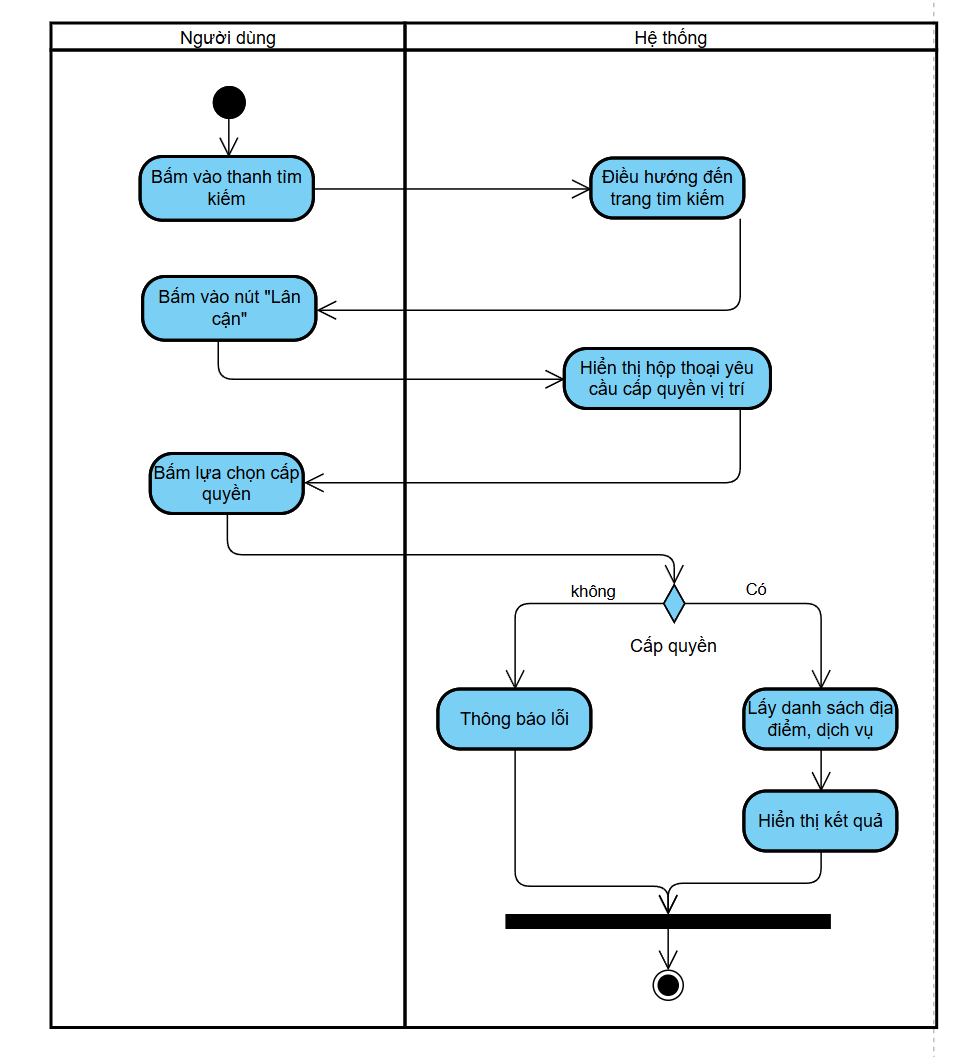
\includegraphics[width=0.5\linewidth]{figures/c3/3-3-7-ad.png} 
    & 
    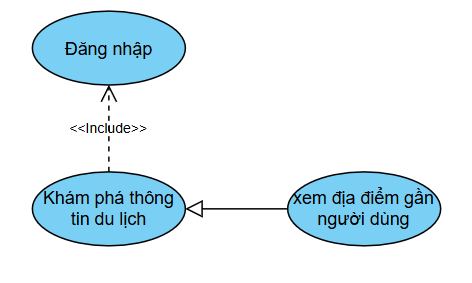
\includegraphics[width=0.45\linewidth]{figures/c3/3-3-7-rd.png} \\ 
    \hline
\end{tabular}


\vspace{0.8cm}

\begin{figure}[H]
    \centering  
    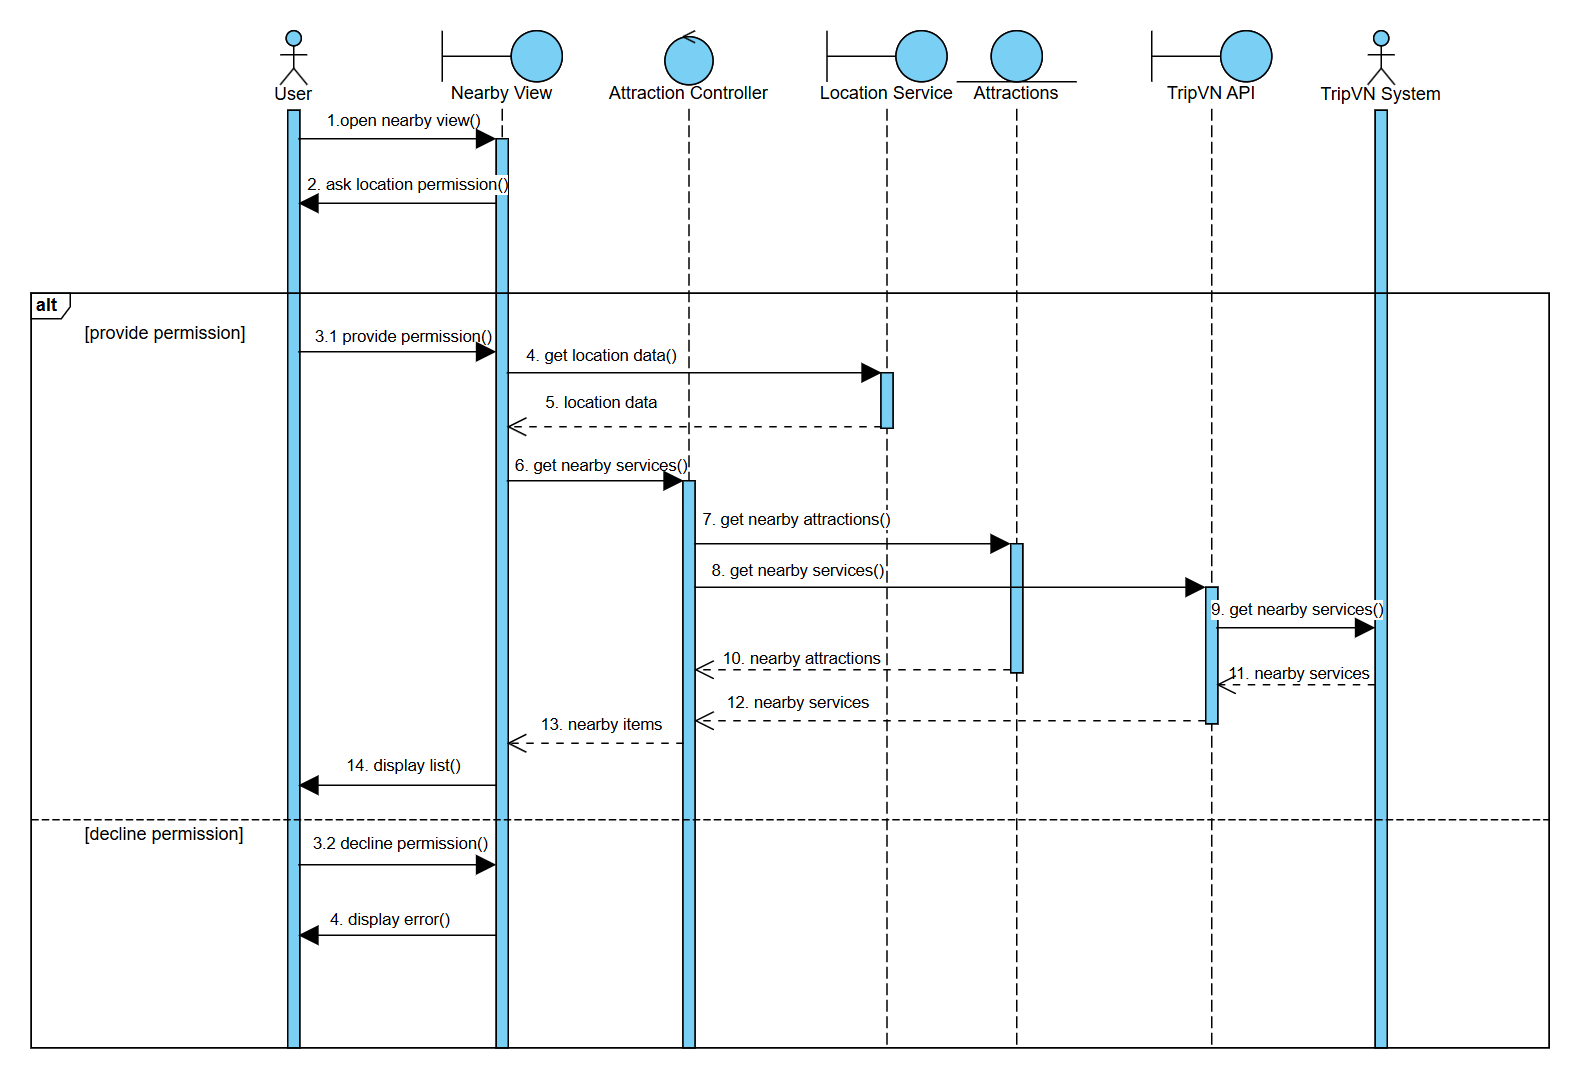
\includegraphics[width=1\textwidth]{figures/c3/3-3-7-sd.png}
    \caption{Biểu đồ tuần tự ca sử dụng xem danh sách địa điểm gần người dùng.}
    \label{fig:3-3-7-sequence-diagram}
\end{figure}